\documentclass[conference]{IEEEtran}
\IEEEoverridecommandlockouts
% The preceding line is only needed to identify funding in the first footnote. If that is unneeded, please comment it out.
\usepackage{cite}
\usepackage{amsmath,amssymb,amsfonts}
\usepackage{algorithmic}
\usepackage{graphicx}
\usepackage{textcomp}
\usepackage{xcolor}
\usepackage{booktabs} % For better table formatting
\usepackage{lipsum}   % For filling largely empty sections if needed, though we rely on your content.

% Standard IEEE BibTeX command
\def\BibTeX{{\rm B\kern-.05em{\\sc i\kern-.025em b}\kern-.08em
    T\kern-.1667em\lower.7ex\hbox{E}\kern-.125emX}}

\begin{document}

\title{AI-Based Stroke Phase Detection and Symmetry Analysis in Competitive Swimming Footage: A Proof of Concept\\
{\footnotesize Progress Report}
}

\author{\IEEEauthorblockN{Daniel Pace}
    \IEEEauthorblockA{\textit{Faculty of Information \& Communication Technology} \\
        \textit{University of Malta}\\
        Msida, Malta \\
        daniel.pace.23@um.edu.mt}
}

\maketitle

\begin{abstract}
    Computer vision analysis in aquatic environments presents unique challenges due to refraction, turbulence, and occlusion, which hinder the accuracy of standard motion tracking systems. 
    This project proposes a non-intrusive AI-based system for stroke phase detection and symmetry analysis in competitive swimming. 
    The core contribution is a novel methodology for dynamic pixel-to-meter scaling using standard lane ropes as calibration objects, addressing the limitations of fixed-camera setups in varying pool environments. 
    This progress report outlines the comparative analysis between traditional computer vision pipelines and Convolutional Neural Networks for feature extraction. 
    It presents the system architecture, preliminary findings on lane rope calibration, and the evaluation plan utilizing both quantitative error metrics and qualitative expert feedback.
\end{abstract}


\section{Introduction}

\subsection{Problem Statement}
Performance analysis in competitive swimming is traditionally reliant on manual observation or expensive, sensor-based systems that can be intrusive to the athlete. 
While computer vision offers a non-intrusive alternative, the aquatic environment introduces significant noise. 
Light refraction at the air-water interface, surface turbulence caused by the swimmer, and occlusions (bubbles and splashes) degrade the quality of visual data~\cite{ahmed2019, giulietti2023}. 
Furthermore, camera distances and angles vary significantly between venues, making consistent metric quantification (e.g., speed in meters/second) difficult without distinct calibration markers.

\subsection{Motivation}
There is a distinct lack of robust, automated systems that can operate on standard broadcast or training footage without requiring complex setup. 
A reliable system capable of extracting metric data from video alone would democratize access to high-level analytics for coaches and athletes. 
The ability to automatically detect stroke phases and analyse left-right symmetry is crucial for identifying technique flaws and preventing injury~\cite{zhou2025, almajnoni2025}.

\subsection{Aims and Objectives}
The primary aim of this project is to develop a Proof of Concept (PoC) system that automates the extraction of swimming metrics. The specific objectives are:
\begin{enumerate}
    \item To implement and compare traditional and CNN-based methods for lane rope detection and segmentation, evaluating their accuracy and robustness across diverse swimming pool environments.
    \item To compute a pixel-to-metre conversion factor using the detected lane rope features, accounting for variations in lane rope design.
    \item To obtain swimmer motion metrics which are dependent on the pixel-to-metre scale, such as swimmer velocity, stroke length, impulse.
    \item To evaluate and compare the performance of the system on datasets containing different swimming strokes, pool environments and camera angles.
\end{enumerate}

\section{Related Work}

\subsection{AI in Sports Analytics}
Artificial Intelligence has revolutionized sports analytics, with mature applications in court-based sports like basketball and tennis~\cite{zhou2025}. 
However, in the domain of aquatic sports, even state-of-the-art AI models struggle due to the environmental complexity. 
Current literature highlights that while pose estimation models perform well on land, their accuracy drops significantly underwater due to the refractive index changes and visual distortions~\cite{giulietti2023, cao2024}.

\subsection{Challenges in Aquatic Computer Vision}
Research indicates that standard tracking algorithms often fail when subject to reflections of water and the rapid occlusion caused by splashing. 
Previous attempts have utilized underwater cameras to mitigate surface refraction, but such setups have limitations of their own, including installation complexity and limited field of view~\cite{tran2024, ahmed2019}.

\subsection{Gap Analysis: Dynamic Scaling}
A critical gap identified in the literature is the lack of automated scaling mechanisms for broadcast footage. Most existing solutions rely on manual calibration or fixed camera positions~\cite{chauhan2025, zuo2021}. 
While World Aquatics regulations mandate specific markings on lane ropes such as the 15m red marker, the design of the rest of the lane rope can vary between manufacturers. 
This project addresses this gap by proposing a calibration method that robustly estimates scale despite these manufacturing variations~\cite{lee2021}.

\section{Proposed Solution}

\subsection{System Architecture}
The proposed solution is structured around a three-stage pipeline, designed to transform raw footage into analytical metrics.

\subsubsection{Stage 1: Lane Rope Calibration}
The foundational innovation of this system is the use of lane ropes for dynamic calibration. 
The system identifies the floating markers on the lane ropes. 
By detecting the periodic colour changes, the system calculates a pixel-to-meter ratio. 
This allows for the normalization of data across different video resolutions and camera zoom levels~\cite{haseeb2018, saputra2021}.

\subsubsection{Stage 2: Feature Extraction}
This stage is the core of the comparative study. 
We are implementing two parallel pipelines to evaluate performance:
\begin{itemize}
    \item Traditional Pipeline: Utilizes Canny Edge Detection and the Hough Transform to identify linear features, such as lane ropes, and basic motion blobs. 
    This approach is computationally inexpensive but susceptible to noise.
    \item CNN-based Pipeline: Utilizing a Neural Net for semantic segmentation and Mask R-CNN for instance segmentation. 
    These models are trained to ignore water turbulence and focus on the structural elements.
\end{itemize}

\subsubsection{Stage 3: System Output}
The final stage aggregates the extracted features to determine stroke count, stroke rate, and symmetry indices. 
The output includes a visual overlay on the original footage and a numerical report for coaches.

\section{Evaluation Plan}

The validation of the proposed system will be conducted through both quantitative and qualitative measures.

\subsection{Quantitative Evaluation}
\begin{itemize}
    \item Axis/Scale Error: The accuracy of the pixel-to-meter conversion will be tested against ground truth measurements of the pool. 
    We will calculate the Mean Absolute Percentage Error (MAPE) of the estimated distances~\cite{holzmann2012}.
    \item Detection Accuracy: For stroke phase detection, we will compute Precision, Recall, and F1-scores, comparing the system's timestamped events against manual annotations by human experts.
\end{itemize}

\subsection{Qualitative Evaluation}
Expert feedback will be solicited from swimming coaches. 
They will assess the utility of the visual overlays and the relevance of the symmetry metrics. 
This feedback will be gathered via a structured survey focusing on the system's potential for real-world training integration.

\section{Conclusion}

This report outlines the implementation achieved thus far and details the remaining steps for the proposed solution. 
For the full project schedule, refer to the Gantt chart located in Appendix A.

\begin{thebibliography}{00}

% 1. Navigational system for visually impaired people
\bibitem{ahmed2019}
S. Ahmed, ``Navigational system for visually impaired people in a swimming pool,'' KTH, Stockholm, Sweden, 2019. [Online]. Available: https://urn.kb.se/resolve?urn=urn:nbn:se:kth:diva-269431

% 2. AI-Based Object Measurement (Cleaned up authors)
\bibitem{chauhan2025}
D. Chauhan, D. Panchal, J. Patel, and D. Bhatt, ``AI-Based Object Measurement Using MiDaS Depth Estimation and MobileNetV3 Edge Detection,'' \emph{International Journal on Science and Technology}, vol. 16, no. 2, p. 3924, Apr. 2025.

% 3. Reference-free video-to-real distance
\bibitem{zuo2021}
F. Zuo, J. Gao, A. Kurkcu, H. Yang, K. Ozbay, and Q. Ma, ``Reference-free video-to-real distance approximation-based urban social distancing analytics amid COVID-19 pandemic,'' \emph{Journal of Transport \& Health}, vol. 21, p. 101032, Jun. 2021.

% 4. Measuring distance with mobile phones
\bibitem{holzmann2012}
C. Holzmann and M. Hochgatterer, ``Measuring distance with mobile phones using single-camera stereo vision,'' in \emph{2012 32nd International Conference on Distributed Computing Systems Workshops}, 2012, pp. 88--93.

% 5. DisNet
\bibitem{haseeb2018}
M. A. Haseeb, J. Guan, D. Ristic-Durrant, and A. Gräser, ``DisNet: A novel method for distance estimation from monocular camera,'' in \emph{10th Planning, Perception and Navigation for Intelligent Vehicles (PPNIV18), IROS}, 2018.

% 6. Experiment on distance measurement
\bibitem{saputra2021}
D. E. Saputra, A. S. M. Senjaya, J. Ivander, and A. W. Chandra, ``Experiment on distance measurement using single camera,'' in \emph{2021 4th International Conference on Information and Communications Technology (ICOIACT)}, 2021, pp. 80--85.

% 7. Category-Level Metric Scale
\bibitem{lee2021}
T. Lee, B.-U. Lee, M. Kim, and I. S. Kweon, ``Category-Level Metric Scale Object Shape and Pose Estimation,'' \emph{IEEE Robotics and Automation Letters}, vol. 6, no. 4, pp. 8575--8582, Oct. 2021.

% 8. Analyzing Swimming Performance (Drone)
\bibitem{tran2024}
T. Tran \emph{et al.}, ``Analyzing Swimming Performance Using Drone Captured Aerial Videos,'' in \emph{Proceedings of the 10th Workshop on Micro Aerial Vehicle Networks, Systems, and Applications}, Minato-ku, Tokyo, Japan, Jun. 2024, pp. 7--12.

% 9. SwimmerNET
\bibitem{giulietti2023}
N. Giulietti, A. Caputo, P. Chiariotti, and P. Castellini, ``SwimmerNET: Underwater 2D Swimmer Pose Estimation Exploiting Fully Convolutional Neural Networks,'' \emph{Sensors}, vol. 23, no. 4, p. 2364, Jan. 2023.

% 10. Pose estimation for swimmers (HRNet)
\bibitem{cao2024}
X. Cao and W. Q. Yan, ``Pose estimation for swimmers in video surveillance,'' \emph{Multimedia Tools and Applications}, vol. 83, no. 9, pp. 26565--26580, Mar. 2024.

% 11. AI in Sport (Narrative Review)
\bibitem{zhou2025}
D. Zhou, J. W. L. Keogh, Y. Ma, R. K. Y. Tong, A. R. Khan, and N. R. Jennings, ``Artificial intelligence in sport: A narrative review of applications, challenges and future trends,'' \emph{Journal of Sports Sciences}, pp. 1--16, 2025.

% 12. Moar: Swimming Style Identification
\bibitem{almajnoni2025}
A. Al-Majnoni, J. Al-Sahli, D. Al-Ahmady, A. Al-Mutairi, A. Alsini, and M. Alharbi, ``Moar: A Swimmer Motion Swimming Style Identification Model using Deep Learning,'' \emph{Engineering, Technology \& Applied Science Research}, vol. 15, no. 1, pp. 19295--19302, Feb. 2025.

\end{thebibliography}
\pagebreak
\section{Appendix A:\@ Project Timeline}

\begin{figure}[h]
    \centering
    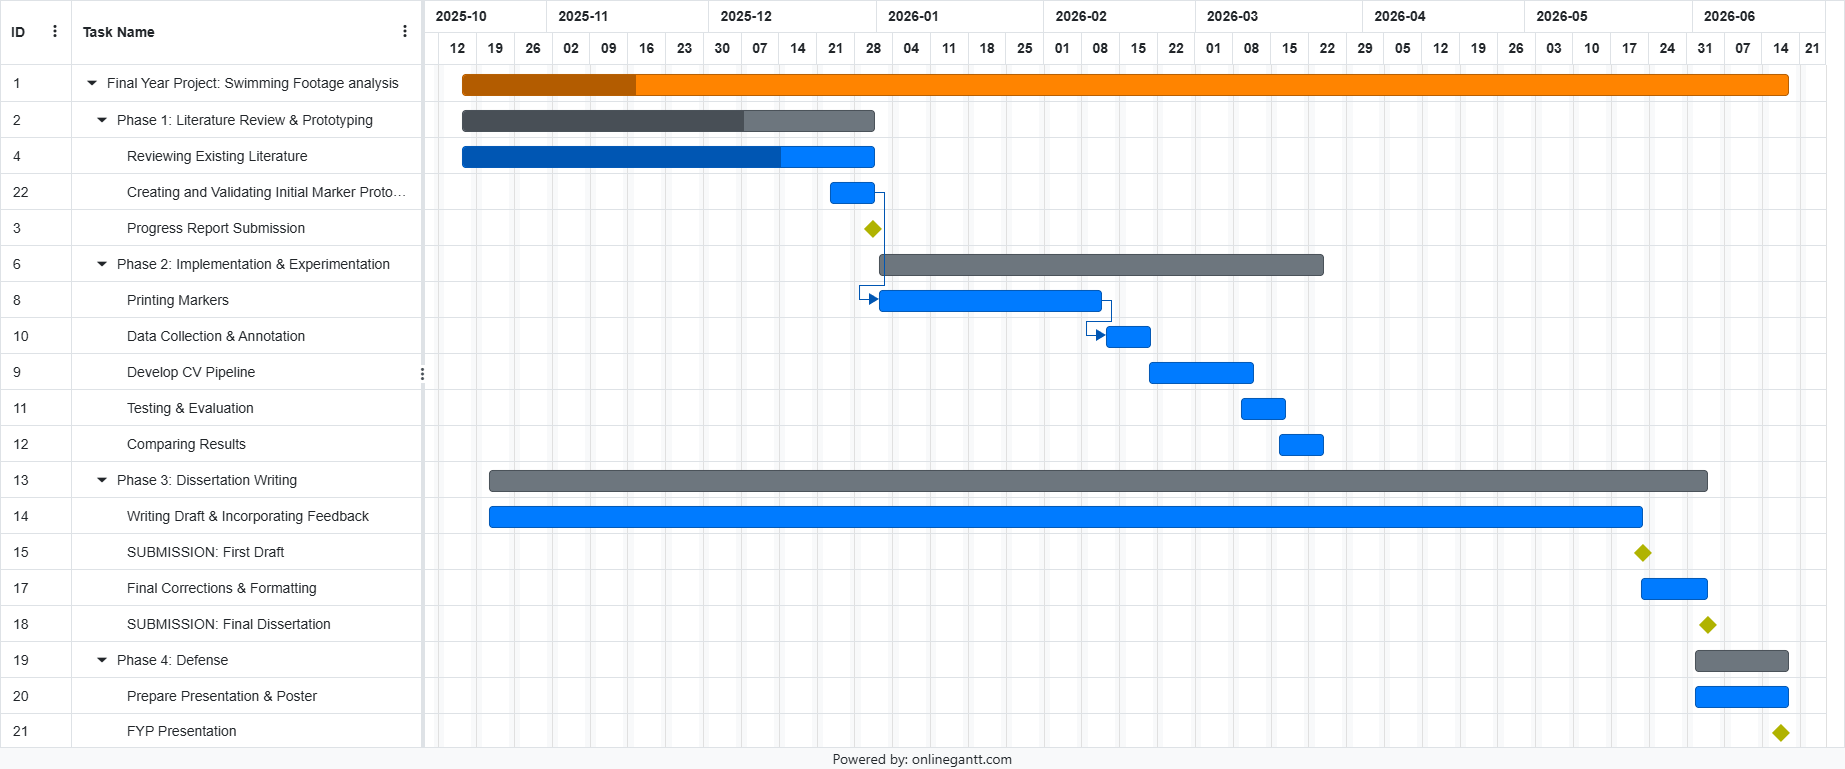
\includegraphics[width=2\linewidth]{Online Gantt 20251208 (1).png}
    \caption{Project timeline and milestones for the AI-based stroke phase detection system.}
    \label{fig:gantt_chart}
\end{figure}

\end{document}

\end{document}